\documentclass[11pt]{article}
\usepackage[utf8]{inputenc}
\usepackage{geometry}
\usepackage{amsfonts}
\usepackage{hyperref}
\usepackage{enumitem}
\usepackage{graphicx}
\usepackage{tabularx}
\usepackage{amsmath}
\usepackage{xcolor}
\usepackage{array}
\usepackage{amsmath}
\usepackage{amssymb}
\usepackage{algorithm}
\usepackage{algorithmic}
\usepackage{graphicx}




\title{
    \textbf{CSE634: Algorithms in Robot Planning} \\ \vspace*{-5pt}
    \textbf{\large{Assignment-2}}
}

\author{Akanksha Singal (2021008)}
\date{\today}

\geometry{a4paper, left=20mm, right=20mm, top=20mm, bottom=20mm}


\begin{document}
\maketitle

\section*{Question-1}
Algorithm $A^*$ selects a path that minimizes $f(n) := g(n) + h(n)$, and always finds an optimal path between two given nodes. However, the number of nodes explored in the process can be very high. Instead, if we modify the cost function to add some bias to the nodes closer to the goal, the number of expanded nodes may be smaller. Suggest a variant of $A^*$ and modify the cost function accordingly such that the above-mentioned bias is added to the nodes closer to the goal.


\subsection*{Given: }
Cost function of A* algorithm as $f(n) := g(n) + h(n)$ where $g(n)$ is the cost to reach node n and $h(n)$ is the estimated cost to reach the goal from node n in the graph.

\subsection*{Objective: }
We want to reduce the total number of states explored by the A* algorithm. 

\subsection*{A* Algorithm: }
A* algorithm incorporates a heuristic estimate of the cost to get to the goal from a given state.
As the estimated cost to reach the goal becomes closer to the true cost to reach, fewer vertices tend to be explored in comparison with Dijkstra’s algorithm.
This would always seem advantageous, but in some problems it is difficult or impossible to find a heuristic that is both efficient to evaluate and provide good search guidance.

\subsection*{Variant of A* Algorithm to reduce number of states explored: }

\subsubsection*{Weighted A* Algorithm}
One effective variant of the A* algorithm that adds bias towards nodes closer to the goal is Weighted A*. 
\newline
The Weighted A* cost function is defined as:
\[
f(n) := g(n) + w \cdot h(n), \quad \text{where } w > 1
\]

In this cost function, we are scaling the cost to reach goal n by a scalar w which increases the bias for reducing the cost to reach the goal. We increase the influence of the heuristic in the cost function. The weight biases the search towards nodes that are heuristically closer to the goal, potentially reducing the number of nodes expanded.

\subsubsection*{Dynamic Weighted A* Algorithm}
This weight can also be set dynamically similar to the learning rate in gradient descent. As the node is closer to the goal, increasing the weight works better. This has been shown in the paper by \cite{chen2021necessary}.
\newline

\textbf{Note:} The weighted variants, both with constant and dynamic weights, of A* with the modified cost function may not always provide an optimal solution. Hence optimality and completeness cannot be guaranteed. The solution obtained depends on the value of the weight in question which can be modified empirically and heuristically. However, finding the right value for the weight remains a difficult task.

Reference for this question can be found here: \href{https://theory.stanford.edu/~amitp/GameProgramming/Variations.html}{\textcolor{blue}{Link}}



\section*{Question 2}
In PRM, the roadmap graph should reflect the connectivity of $C_{\text{free}}$ in the workspace. In a 3-dimensional workspace, the time required for adding a node (or, sample) is huge compared to checking if that sample is obstacle-free or not. So, it is important to add as few nodes as possible in the graph. Clearly, we do not need a sample that collides with an obstacle, we also do not want many samples in large open regions. We DO WANT samples close to the samples in difficult regions (e.g., with complex obstacles). Suggest a suitable sample distribution strategy that will capture the above. Design an algorithm for obtaining the sample distribution suggested by you.

\subsection*{Objective: }
\begin{itemize}
  \item \textbf{Avoid Sampling within Obstacles:} Ensure that no samples are placed inside obstacles.
  \item \textbf{Reduce Oversampling in Open Regions:} Limit the number of samples in large open spaces where connectivity is easily maintained.
  \item \textbf{Increase Sampling Near Obstacles:} We DO WANT samples close to the samples in difficult regions
\end{itemize}

\subsection*{Solution}
One way to achieve this by using an Obstacle Potential Field to bias the sampling distribution without placing samples inside the obstacles.

\subsection*{Obstacle Potential Field}
Points closer to obstacles have higher potential and thus a higher chance of being accepted. Within the obstacle, the potential field is ideally infinite. We increase the density of samples near obstacles while reducing it in open spaces. This approach ensures more samples are placed in complex regions, while less in the free open regions. 

A sample potential field of the configuration space looks like the image given.

\begin{center}
    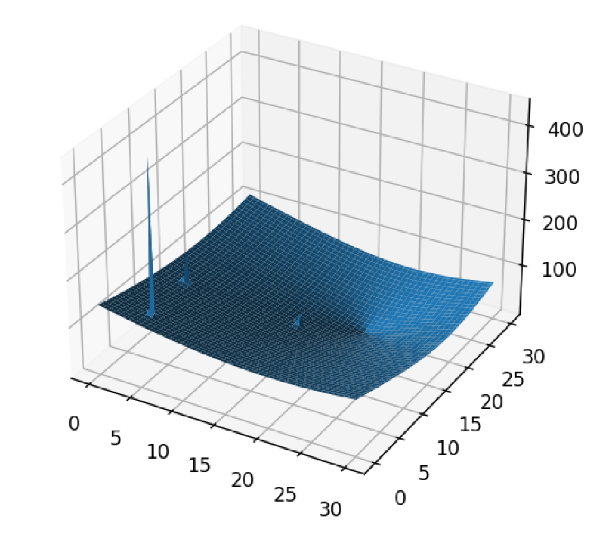
\includegraphics[width=0.5\textwidth]{artificial_potential_field.png}
\end{center}

\subsection*{Algorithm for obtaining the sample distribution}

Since, checking if the point is within the obstacle or not is easier, we sample points using uniform distribution. We check that if the point is collision free and higher than a certain threshold of potential field then we add it to our vertex list. This approach is referenced from \cite{op-prm}.


\begin{algorithm}
\caption{Sampling Algorithm with Potential Field Values}
\begin{algorithmic}[1]
\STATE Obtain a sampling point \(q\) using a uniform distribution;
\STATE Calculate the potential field value \(U_q\) of \(q\);
\IF{\(U_q > U_0\)}
    \STATE Add \(q\) to vertex set \(V\)\;
\ENDIF

\end{algorithmic}
\end{algorithm}


\subsection*{Sampling Using Probabilities}
Modifying the above approach, We can propose using potential fields to define a RV Q with probability distribution that of the potential field.
Higher the potential field, higher the probability of sampling points q. Except when the potential field is infinite (ideally) in case of obstacle or higher than a certain threshold value say $U_{thresh}$, then probability is 0. 
\newline
\newline
We define the potential field \( U(q) \) over the configuration space \( C \) with the following properties:
\begin{itemize}
    \item \textbf{High Potential Near Obstacles:} \( U(q) \) is higher in regions close to obstacles.
    \item \textbf{Infinite Potential Inside Obstacles:} \( U(q) = \infty \) for all \( q \in C_{\text{obs}} \).
\end{itemize}

We define a probability density function \( p(q) \) over the free configuration space \( C_{\text{free}} \) based on the potential field \( U(q) \):

\[
p(q) =
\begin{cases} 
    \frac{U(q)}{Z} & \text{if } q \in C_{\text{free}} \text{ and } U(q) \leq U_{\text{thresh}}, \\
    0 & \text{if } q \in C_{\text{obs}} \text{ or } U(q) > U_{\text{thresh}},
\end{cases}
\]

where \( Z \) is the normalization constant ensuring \( p(q) \) is a valid probability density function:

\[
Z = \int_{C_{\text{free}}} U(q) \, dq.
\]



\bibliographystyle{plain}
\bibliography{references}

\end{document}